\documentclass[10pt,a4paper,twocolumn]{article}

\usepackage[a4paper,top=0.75in,bottom=0.85in,left=0.65in,right=0.65in]{geometry}
\usepackage[utf8]{inputenc}
\usepackage[T1,T5]{fontenc}
\usepackage{lmodern}
\usepackage{microtype}

\usepackage{amsmath,amssymb,amsthm}
\newtheorem{definition}{Definition}
\newtheorem{theorem}{Theorem}
\usepackage{xurl}
\usepackage{graphicx}
\usepackage{float}
\usepackage{xcolor}
\usepackage{booktabs}
\usepackage{tabularx}
\usepackage{array}
\usepackage{makecell}
\usepackage{enumitem}
\usepackage{listings}
\usepackage{algorithm}
\usepackage{algpseudocode}
\floatstyle{boxed}
\restylefloat{algorithm}
\usepackage[font=footnotesize,labelfont=bf]{caption}
\usepackage{titlesec}
\usepackage[colorlinks=true,linkcolor=blue,citecolor=blue,urlcolor=blue]{hyperref}
\usepackage[nameinlink]{cleveref}

% Refined Section Typography for Compact 2-column Research Paper
\titleformat{\section}
  {\normalfont\fontsize{10.5pt}{12pt}\bfseries}
  {\thesection}{0.6em}{}
\titlespacing*{\section}{0pt}{8pt plus 2pt minus 2pt}{3pt plus 1pt minus 1pt}

\titleformat{\subsection}
  {\normalfont\fontsize{9.8pt}{11pt}\bfseries}
  {\thesubsection}{0.5em}{}
\titlespacing*{\subsection}{0pt}{6pt plus 1.5pt minus 1.5pt}{2pt plus 1pt minus 1pt}

\titleformat{\subsubsection}
  {\normalfont\fontsize{9.2pt}{10.5pt}\itshape\bfseries}
  {\thesubsubsection}{0.4em}{}
\titlespacing*{\subsubsection}{0pt}{4pt plus 1pt minus 1pt}{1.5pt plus 0.5pt minus 0.5pt}

% Header and Footer Management
\usepackage{fancyhdr}
\pagestyle{fancy}
\setlength{\headheight}{13pt}

\setlength{\parindent}{1em}
\setlength{\parskip}{0pt}
\setlength{\emergencystretch}{1.5em}
\setlist[itemize]{leftmargin=1.2em,itemsep=0.1em,topsep=0.15em}
\setlist[enumerate]{leftmargin=1.3em,itemsep=0.1em,topsep=0.15em}

% Header & Footer
\fancyhf{}
\lhead{\footnotesize\textsl{CS420: Intro to AI -- [S04] LIME \& SHAP}}
\rhead{\footnotesize\textsl{VNUHCM - University of Science}}
\cfoot{\thepage}
\renewcommand{\headrulewidth}{0.4pt}
\renewcommand{\footrulewidth}{0pt}

% Title, Authors, and Metadata
\title{\textbf{\fontsize{13.5pt}{15.5pt}\selectfont Does an Accurate Prediction Come with a Reliable Explanation?}\\[0.25em]
\fontsize{11pt}{13pt}\selectfont\textbf{A Comparative Study of LIME and SHAP}}

\author{
    \textbf{Nguyễn Gia Hào} \\
    \texttt{24125008} \\
    \small APCS -- Faculty of Information Technology \\
    \small VNUHCM - University of Science
    \and
    \textbf{Phạm Hữu Nam} \\
    \texttt{24125015} \\
    \small APCS -- Faculty of Information Technology \\
    \small VNUHCM - University of Science
    \and
    \textbf{Nguyễn Hữu Phước} \\
    \texttt{24125018} \\
    \small APCS -- Faculty of Information Technology \\
    \small VNUHCM - University of Science
}
\date{\small Instructor: Dr. Nguyễn Ngọc Thảo}

% ============ DOCUMENT ============
\begin{document}

\twocolumn[
  \begin{@twocolumnfalse}
    \maketitle
    \begin{abstract}
Artificial intelligence models are seeing widespread adoption across critical domains such as healthcare, finance, and criminal justice. Understanding the reasons behind their predictions is essential for establishing trust and reliability. This seminar paper investigates two foundational post-hoc Explainable Artificial Intelligence (XAI) methods: \textbf{Local Interpretable Model-agnostic Explanations (LIME)} and \textbf{SHapley Additive exPlanations (SHAP)}. Centered on the guiding research question: \textit{``Does a highly accurate prediction necessarily come with a reliable explanation?''}, this work covers:
(i)~\textbf{Conceptual Foundations:} Positioning post-hoc interpretability within a four-dimensional XAI taxonomy, distinguishing intrinsic from post-hoc mechanisms and local from global scopes;
(ii)~\textbf{Theoretical Formulations \& Worked Examples:} Detailing the exact optimization objectives and underlying game-theoretic axioms of LIME and SHAP, supported by step-by-step numerical calculations on an illustrative model;
(iii)~\textbf{Empirical Demonstration:} Evaluating both methods on the Breast Cancer Wisconsin dataset using a Random Forest classifier across confident, borderline, and conflicting prediction cases;
(iv)~\textbf{Runtime \& Instability:} Benchmarking computational latency across TreeSHAP, KernelSHAP, and LIME, while demonstrating explanation instability in LIME caused by stochastic sampling; and
(v)~\textbf{Faithfulness \& Limitations:} Evaluating explanation faithfulness via empirical feature-deletion experiments and addressing why post-hoc attributions must not be interpreted as causal effects.

\vspace{0.8em}
\noindent\textbf{Keywords:} Explainable AI (XAI), LIME, SHAP, KernelSHAP, TreeSHAP, Shapley Values, Local Accuracy, Consistency, Model Faithfulness.
\end{abstract}

    \vspace{1.2em}
  \end{@twocolumnfalse}
]

\section{Introduction}
\label{sec:introduction}

Modern machine learning systems have achieved remarkable performance across diverse analytical benchmarks. However, the most accurate predictors---such as deep neural networks or ensemble tree architectures---even domain experts struggle to interpret, creating a tension between accuracy and interpretability.

In critical applications such as clinical oncology, autonomous driving, and financial risk assessment, high predictive accuracy alone is insufficient. Stakeholders require transparent, verifiable rationales before decisions can be safely operationalized~\cite{BARREDOARRIETA202082}. Explainable Artificial Intelligence (XAI) has emerged to bridge this fundamental tension between predictive capacity and human interpretability. Among post-hoc local explanation frameworks, LIME~\cite{ribeiro-etal-2016-trust} and SHAP~\cite{NIPS2017_8a20a862} have become standard industry and research benchmarks. Despite their ubiquity, practitioner reliance on these tools often presumes that high predictive accuracy naturally guarantees fidelity and reliability in the accompanying explanations.

\subsection{Research Question}
\label{sec:guiding-question}

Motivated by this gap, this seminar investigates the central question: \textit{``Does a highly accurate prediction necessarily come with a reliable explanation?''} 

To answer this question, we systematically examine LIME and SHAP across both theoretical foundations and empirical behavior:
\begin{itemize}[leftmargin=1.2em, itemsep=1.5pt]
    \item \textbf{Conceptual Foundations:} Clarifying where post-hoc local methods stand within the broader XAI taxonomy, distinguishing intrinsic from post-hoc models and local from global scopes.
    \item \textbf{Theoretical Formulations \& Worked Examples:} Walking through the exact mathematical objectives and game-theoretic foundations of both methods, accompanied by step-by-step numerical calculations on an illustrative example.
    \item \textbf{Empirical Demonstration:} Evaluating explanations produced for a Random Forest classifier on the Breast Cancer Wisconsin dataset across confident, borderline, and conflicting prediction scenarios.
    \item \textbf{Faithfulness \& Limitations:} Analyzing explanation stability across random seeds, runtime trade-offs, empirical faithfulness via feature deletion, and why post-hoc attributions must not be conflated with causal effects.
\end{itemize}



\section{Background and Related Work}
\label{sec:background}

\subsection{Taxonomy of Explainable AI (XAI)}
\label{sec:taxonomy}

Explainable Artificial Intelligence (XAI) addresses the tension between model accuracy and interpretability. To establish a structured foundation, the literature synthesizes XAI techniques across primary operational dimensions~\cite{BARREDOARRIETA202082, 10.1016/j.neucom.2024.128111}:

\subsubsection{Interpretability vs.\ Explainability}
The boundary between interpretability and explainability remains an active subject of discussion in the machine learning literature. As surveyed comprehensively by Mersha et al.~\cite{10.1016/j.neucom.2024.128111}, although these two terms are frequently conflated in casual discourse, most studies agree that they denote related but distinct concepts:
\begin{itemize}[leftmargin=1.5em, itemsep=2pt]
    \item \textbf{Interpretability (How the model works):} Refers to the inherent capacity of a system to be understood directly by human observers without external aids. An interpretable model possesses intrinsic algorithmic transparency, allowing stakeholders to trace internal calculations and understand the complete decision mechanics (e.g., shallow decision trees or sparse linear models).
    \item \textbf{Explainability (Why the model predicts):} Pertains to the ability of an external, secondary interface to clarify and justify the outputs of an opaque system. Explainability does not require the underlying architecture to be transparent; instead, it relies on post-hoc surrogate methods to articulate the rationale behind a decision in human-understandable terms.
\end{itemize}
In short, interpretability concerns the internal mechanics of a model, whereas explainability focuses on rationalizing specific predictions. Within this conceptual division, LIME and SHAP serve fundamentally as post-hoc tools for explainability.

\subsubsection{Local vs.\ Global Explanations}
Depending on the scope of the explanation, XAI techniques generally operate at either a local or a global level:
\begin{itemize}[leftmargin=1.2em, itemsep=1.5pt]
    \item \textbf{Local Explanations:} Focus on explaining a single prediction for an individual instance. Rather than describing how the model behaves everywhere, a local explanation identifies which specific features drove the decision for that particular case. For example, in clinical diagnosis, a local explanation reveals why a specific patient was assigned a 94\% probability of malignancy (e.g., due to extreme tumor radius and irregular texture).
    \item \textbf{Global Explanations:} Aim to describe the overall behavior of the model across the entire dataset. A global explanation provides a high-level summary of how the model makes decisions in general, revealing overall feature rankings and broader decision patterns (e.g., determining which clinical indicators are universally most influential across all patients).
\end{itemize}
While LIME was originally formulated strictly for local explanations, SHAP values computed locally for individual instances can be aggregated across the entire dataset to provide consistent global insights.

\subsubsection{Ante-hoc vs.\ Post-hoc Interpretability}
The critical difference between ante-hoc and post-hoc techniques is the stage of implementation relative to model training~\cite{BARREDOARRIETA202082, 10.1016/j.neucom.2024.128111}:
\begin{itemize}[leftmargin=1.2em, itemsep=1.5pt]
    \item \textbf{Ante-hoc Methods:} Employed during the model design and training stages to ensure that the system is transparent and directly understandable by construction (e.g., shallow decision trees, Generalized Additive Models, and Bayesian models).
    \item \textbf{Post-hoc Methods:} Employed after the model has been trained and its parameters frozen. Post-hoc techniques do not modify the original architecture; instead, they construct external explanation mechanisms to elucidate the decision-making process of opaque models (such as deep neural networks and Random Forests).
\end{itemize}
Both LIME and SHAP are foundational post-hoc explanation techniques, designed to interrogate already-trained black-box models.

\subsubsection{Model-Specific vs.\ Model-Agnostic Post-hoc Explanations}
As categorized by Barredo Arrieta et al.~\cite{BARREDOARRIETA202082} and surveyed by Mersha et al.~\cite{10.1016/j.neucom.2024.128111}, post-hoc explanation techniques branch into two distinct operational paradigms:
\begin{itemize}[leftmargin=1.2em, itemsep=1.5pt]
    \item \textbf{Model-Specific Methods:} Techniques designed specifically for a single model family by taking advantage of its internal structure. Because they have direct access to internal components (such as split thresholds of decision trees or neural network weights), they are computationally efficient. For instance, \textbf{TreeSHAP} inspects tree branches directly to calculate Shapley values in polynomial time, but only works on tree-based models.
    \item \textbf{Model-Agnostic Methods:} Universal techniques that can be applied to \textit{any} machine learning model without knowing what is inside. They treat the model as a strict black box, observing only how predictions change when input values are slightly perturbed. \textbf{LIME} and \textbf{KernelSHAP} belong to this category.
\end{itemize}

\subsection{LIME}
\label{sec:review-lime}

In \textit{``Why Should I Trust You?'': Explaining the Predictions of Any Classifier}~\cite{ribeiro-etal-2016-trust}, Ribeiro, Singh, and Guestrin formalized Local Interpretable Model-agnostic Explanations (LIME). The core philosophy of LIME asserts that although a decision surface $f: \mathbb{R}^d \rightarrow [0, 1]$ may be globally non-linear and intractable, it is locally smooth within an $\epsilon$-ball centered at a target query point $x$. Consequently, $f$ can be faithfully approximated in that localized region by an interpretable surrogate model $g \in G$.

LIME operationalizes this insight through stochastic perturbation:
\begin{enumerate}[leftmargin=1.2em, itemsep=1.5pt]
    \item \textbf{Perturbation Sampling:} Draws synthetic instances $z'$ uniformly or via normal perturbation around the query instance in an interpretable representation space (e.g., binary word indicators or superpixel segments).
    \item \textbf{Locality Weighting:} Maps perturbed instances back to original feature space $z = h_x(z')$ and weights each perturbation using an exponential distance kernel $\pi_x(z) = \exp(-D(x, z)^2 / \sigma^2)$.
    \item \textbf{Surrogate Model Fitting:} Solves a weighted penalization loss objective, optimizing the surrogate parameters to minimize local approximation error while constraining complexity $\Omega(g)$.
\end{enumerate}

\subsection{SHAP}
\label{sec:review-shap}

In \textit{A Unified Approach to Interpreting Model Predictions}~\cite{NIPS2017_8a20a862}, Lundberg and Lee addressed a major fragmentation in the XAI literature: prior to 2017, numerous interpretability methods existed (such as LIME, DeepLIFT, and Layer-Wise Relevance Propagation), yet there was no common theoretical framework to compare their mathematical guarantees.

The fundamental insight of SHAP is twofold:
\begin{enumerate}[leftmargin=1.2em, itemsep=1.5pt]
    \item \textbf{A Unified Class of Additive Explanations:} Lundberg and Lee proved that several prominent local explanation methods can all be formalized as \textit{additive feature attribution methods}---approximating the model locally as a linear sum of feature contributions.
    \item \textbf{Game-Theoretic Optimality (Shapley Values):} Drawing from cooperative game theory~\cite{shapley1953value}, SHAP demonstrates that assigning credit using classical Shapley values is the \textit{only} formulation that guarantees three essential fairness properties:
    \begin{itemize}[leftmargin=1.2em, itemsep=1pt]
        \item \textit{Local Accuracy (Efficiency):} The sum of all feature contributions, combined with the baseline average prediction, exactly recovers the actual model output.
        \item \textit{Missingness:} A feature that is completely absent from the input receives zero contribution.
        \item \textit{Consistency (Monotonicity):} If a model changes such that a feature's marginal contribution increases (or stays the same) regardless of other features, its assigned importance will never decrease.
    \end{itemize}
\end{enumerate}

To make Shapley values computationally tractable in practice, Lundberg and Lee initially introduced \textbf{KernelSHAP}~\cite{NIPS2017_8a20a862}, a model-agnostic approximation based on weighted linear regression. Subsequently, Lundberg et al.~\cite{lundberg2018consistent} proposed \textbf{TreeSHAP}, a dedicated model-specific algorithm that computes exact Shapley values for tree ensembles in polynomial time.

\subsection{Taxonomic Positioning of LIME and SHAP}
\label{sec:taxonomic-positioning}

Synthesizing the theoretical frameworks of Ribeiro et al.~\cite{ribeiro-etal-2016-trust} and Lundberg and Lee~\cite{NIPS2017_8a20a862} against the taxonomy of Mersha et al.~\cite{10.1016/j.neucom.2024.128111}:
\begin{itemize}[leftmargin=1.2em, itemsep=1.5pt]
    \item \textbf{LIME} occupies the quadrant of \textit{Post-hoc, Local, Model-Agnostic, Surrogate-based} explainability.
    \item \textbf{SHAP (KernelSHAP)} is \textit{Post-hoc, Local, Model-Agnostic, Axiomatic-attribution} explainability.
    \item \textbf{TreeSHAP} transitions into \textit{Post-hoc, Local, Model-Specific (Tree-Ensemble)} explainability, exchanging model agnosticism for exact determinism and orders-of-magnitude computational speedups.
\end{itemize}

\section{Explanation Methods}
\label{sec:method}

\subsection{Mathematical Formulation of LIME}
\label{sec:math-lime}

LIME operationalizes a three-stage computational workflow:
\begin{center}
    \textbf{Stochastic Perturbation $\longrightarrow$ Locality-based Kernel Weighting $\longrightarrow$ Fitting Interpretable Surrogate}
\end{center}

Formally, the explanation $\xi(x)$ for instance $x$ is defined via the constrained optimization objective:
\begin{equation}
    \xi(x) = \arg\min_{g \in G} \left[ \mathcal{L}(f, g, \pi_x) + \Omega(g) \right]
    \label{eq:lime-objective}
\end{equation}

\subsection{Definitions of Symbols and Modeling Assumptions}
\begin{itemize}
    \item $f: \mathbb{R}^d \rightarrow [0, 1]$: The fixed, pre-trained black-box predictive model (e.g., probability output of an ensemble classifier).
    \item $x \in \mathbb{R}^d$: The original instance in continuous/discrete feature space being explained, mapped to binary representation $x' \in \{0, 1\}^M$ indicating feature presence.
    \item $g \in G$: The interpretable surrogate model. Typically, $G$ is the family of sparse linear models:
    \begin{equation}
        g(z') = w_0 + \sum_{j=1}^M w_j z'_j = w_0 + w^T z'
    \end{equation}
    where $w_j \in \mathbb{R}$ quantifies the local attribution of feature $j$.
    \item $\pi_x(z)$: The proximity measure defining the local neighborhood around $x$. Using an exponential kernel over a distance metric $D(x, z)$ (e.g., Euclidean or cosine distance):
    \begin{equation}
        \pi_x(z) = \exp\left( - \frac{D(x, z)^2}{\sigma^2} \right)
        \label{eq:lime-kernel}
    \end{equation}
    where $\sigma > 0$ denotes the kernel width hyperparameter determining the effective neighborhood volume.
    \item $\mathcal{L}(f, g, \pi_x)$: The local unfaithfulness loss measuring how poorly $g$ approximates $f$ in the neighborhood defined by $\pi_x$:
    \begin{equation}
        \mathcal{L}(f, g, \pi_x) = \sum_{z, z' \in \mathcal{Z}} \pi_x(z) \left( f(z) - g(z') \right)^2
    \end{equation}
    where $\mathcal{Z}$ is a dataset of synthetic perturbations sampled around $x$.
    \item $\Omega(g)$: The complexity penalty enforcing human interpretability (e.g., restricting the number of non-zero coefficients via $\Omega(g) = \infty \cdot \mathbb{I}(\|w\|_0 > K)$ or via $L_1$ Lasso regularization).
\end{itemize}

\subsection{Mathematical Formulation of SHAP}
\label{sec:math-shap}

\subsubsection{Additive Feature Attribution Methods}
Let $f$ denote the original predictive model to be explained, and let $g$ represent an explanation model. Following the framework formalized by Lundberg and Lee~\cite{NIPS2017_8a20a862}, we focus on local explanation methods designed to explain a specific prediction $f(x)$ for a single input instance $x \in \mathbb{R}^d$, as originally popularized by LIME~\cite{ribeiro-etal-2016-trust}.

Explanation models frequently operate on a \textit{simplified input representation} $x'$, which maps to the original input space through a mapping function $x = h_x(x')$. Local methods aim to ensure that the surrogate matches the black box locally, namely $g(z') \approx f(h_x(z'))$ whenever $z' \approx x'$ (with $h_x(x') = x$, even if $x'$ contains less information than $x$, because $h_x$ is specific to the current query input $x$).

\begin{definition}[Additive Feature Attribution Methods]
\label{def:additive-attribution}
An explanation model $g$ is an additive feature attribution method if it is defined as a linear function of binary variables:
\begin{equation}
    g(z') = \phi_0 + \sum_{i=1}^M \phi_i z'_i
    \label{eq:shap-additive}
\end{equation}
where $z' \in \{0, 1\}^M$ is a binary vector indicating the presence ($z'_i = 1$) or absence ($z'_i = 0$) of simplified feature $i$, $M$ is the number of simplified input features, and $\phi_i \in \mathbb{R}$ quantifies the effect attributed to feature $i$. The constant $\phi_0 = f_x(\emptyset) = \mathbb{E}[f(X)]$ represents the model's base expected prediction when no feature information is provided.
\end{definition}

Methods matching this definition attribute an effect $\phi_i$ to each feature, such that summing the effects of all feature attributions approximates the original model output $f(x)$ for the current input (where all features are present, $z'_i = 1$). Crucially, Lundberg and Lee~\cite{NIPS2017_8a20a862} demonstrated that widely adopted local explanation frameworks---including LIME, DeepLIFT, and Layer-Wise Relevance Propagation---all match this formulation, differing primarily in how they define the mapping $h_x$, the neighborhood kernel, and their specific attribution coefficients.

\subsubsection{Shapley Values and the Characteristic Function}
Originating from cooperative game theory~\cite{shapley1953value}, the Shapley value divides the total game payout fairly among players according to their marginal contributions. Transferred to machine learning, features act as players, and the model prediction serves as the payout:
\begin{equation}
    \phi_i(f, x) = \sum_{S \subseteq F \setminus \{i\}} \frac{|S|!(|F| - |S| - 1)!}{|F|!} \left[ f_x(S \cup \{i\}) - f_x(S) \right]
    \label{eq:shapley-formula}
\end{equation}
where:
\begin{itemize}[leftmargin=1.5em, itemsep=2pt]
    \item $F = \{1, 2, \dots, M\}$ is the grand coalition containing all $M$ available features (with cardinality $|F| = M$).
    \item $S \subseteq F \setminus \{i\}$ is a sub-coalition excluding feature $i$, with cardinality $|S|$.
    \item The combinatorial factor $\frac{|S|!(|F| - |S| - 1)!}{|F|!} = \frac{|S|!(M - |S| - 1)!}{M!}$ denotes the probability that feature $i$ joins coalition $S$ when all features are ordered uniformly at random.
    \item $f_x(S)$ is the characteristic value function representing the model's conditional expected prediction when only the subset of features in $S$ is known ($z'_i = 1$ for $i \in S$ and $z'_i = 0$ for $i \notin S$). To compute $f(h_x(z'))$ when black-box models cannot natively evaluate missing inputs, the conditional expectation can be approximated across successive simplifying assumptions:
    \begin{align}
        f(h_x(z')) &= \mathbb{E}[f(X) \mid X_S = x_S] && \text{\scriptsize(Simplified input mapping)} \label{eq:approx-cond} \\
        &= \mathbb{E}_{X_{\bar{S}} \mid X_S = x_S}\left[ f(x_S, X_{\bar{S}}) \right] && \text{\scriptsize(Expectation over absent features $X_{\bar{S}} \mid X_S$)} \label{eq:approx-marginal} \\
        &\approx \mathbb{E}_{X_{\bar{S}}}\left[ f(x_S, X_{\bar{S}}) \right] = \int f(x_S, x_{\bar{S}}) \, p(x_{\bar{S}}) \, dx_{\bar{S}} && \text{\scriptsize(Feature independence assumption)} \label{eq:approx-indep} \\
        &\approx f\left( \left[ x_S, \mathbb{E}[X_{\bar{S}}] \right] \right) && \text{\scriptsize(Model linearity assumption)} \label{eq:approx-lin}
    \end{align}
    where $x_S$ denotes the observed values for features present in coalition $S$, and $\bar{S} = F \setminus S$ denotes the set of absent features. While \Cref{eq:approx-indep} is standardly adopted in KernelSHAP via empirical background sampling, \Cref{eq:approx-lin} further assumes model linearity to replace missing features simply by their mean reference values.
\end{itemize}

\subsubsection{Axiomatic Foundation and Theorem 1}
\label{sec:shap-axioms}

The connection between additive feature attributions and cooperative game theory is formalized by the following uniqueness result:
\begin{theorem}[Uniqueness of Shapley Attributions]
\label{thm:shapley-uniqueness}
Only one possible explanation model $g$ follows Definition~\ref{def:additive-attribution} and simultaneously satisfies Properties 1, 2, and 3: the attribution values $\phi_i(f, x)$ are uniquely given by the classical Shapley value formula defined in \Cref{eq:shapley-formula}.
\end{theorem}

Grounded in cooperative game theory~\cite{shapley1953value}, Theorem~\ref{thm:shapley-uniqueness} establishes that for a given mapping $h_x$, any additive feature attribution method not based on Shapley values necessarily violates either Local Accuracy or Consistency (as missingness is already respected by most methods).

The three foundational properties governing this uniqueness result are defined as follows:
\begin{enumerate}[leftmargin=1.5em, itemsep=2pt]
    \item \textbf{Property 1 (Local Accuracy / Efficiency):} The explanation model $g(x')$ matches the original black-box model $f(x)$ when $x = h_x(x')$:
    \begin{equation}
        f(x) = g(x') = \phi_0 + \sum_{i=1}^M \phi_i x'_i
        \label{eq:local-accuracy}
    \end{equation}
    where $\phi_0 = f_x(\emptyset)$ is the base model output. When all features are present in the query instance ($x'_i = 1$ for all $i$), this ensures that the sum of all attributions plus the baseline exactly recovers the prediction $f(x)$.
    \item \textbf{Property 2 (Missingness):} Features missing in the simplified input representation receive zero allocated impact:
    \begin{equation}
        x'_i = 0 \implies \phi_i = 0
        \label{eq:missingness}
    \end{equation}
    If the simplified inputs represent feature presence, any feature absent in the original input is guaranteed to have no influence on the explanation.
    \item \textbf{Property 3 (Consistency / Monotonicity):} Let $f$ and $f'$ be two predictive models. If a feature's marginal contribution in model $f'$ is greater than or equal to that in model $f$ across all possible coalitions:
    \begin{equation}
        f'_x(S \cup \{i\}) - f'_x(S) \ge f_x(S \cup \{i\}) - f_x(S) \quad \forall S \subseteq F \setminus \{i\}
        \label{eq:consistency}
    \end{equation}
    then its allocated attribution cannot decrease: $\phi_i(f', x) \ge \phi_i(f, x)$.
\end{enumerate}

\subsubsection{Model-Agnostic Approximation: KernelSHAP}
\label{sec:kernelshap-mechanism}

Direct computation of \Cref{eq:shapley-formula} requires evaluating $2^M$ coalitions. For datasets with moderate to high dimensionality (such as the 30 features in Breast Cancer Wisconsin, requiring $2^{30} \approx 10^9$ evaluations), exact combinatorial summation is computationally impossible.

At first glance, the weighted regression formulation of LIME in \Cref{eq:lime-objective} appears fundamentally distinct from the combinatorial Shapley formula in \Cref{eq:shapley-formula}. However, because linear LIME belongs to the family of additive feature attribution methods (Definition~\ref{def:additive-attribution}), Theorem~\ref{thm:shapley-uniqueness} guarantees that Shapley values represent the unique set of coefficients that satisfy Local Accuracy, Missingness, and Consistency. In original LIME~\cite{ribeiro-etal-2016-trust}, the loss function $L$, weighting kernel $\pi_x$, and complexity penalty $\Omega$ are chosen heuristically (e.g., exponential distance kernels and Ridge/Lasso regularization), causing LIME to violate Local Accuracy and Consistency.

To resolve this limitation, Lundberg and Lee~\cite{NIPS2017_8a20a862} solved the inverse problem: deriving the exact analytical forms of $L$, $\pi_x$, and $\Omega$ that force the linear regression solution to recover exact Shapley values:

\begin{theorem}[Shapley Kernel]
\label{thm:shapley-kernel}
Under Definition~\ref{def:additive-attribution}, the unique choices of regularization penalty $\Omega(g)$, weighting kernel $\pi_x(z')$, and squared loss function $L$ that ensure the solution to the surrogate optimization objective matches the Shapley values and satisfies Properties 1 through 3 are:
\begin{align}
    \Omega(g) &= 0 \label{eq:kernelshap-reg} \\
    \pi_x(z') &= \frac{M - 1}{\binom{M}{|z'|} \, |z'| \, (M - |z'|)} \label{eq:shap-kernel} \\
    L(f, g, \pi_x) &= \sum_{z' \in \mathcal{Z}} \left[ f(h_x(z')) - g(z') \right]^2 \pi_x(z') \label{eq:kernelshap-loss}
\end{align}
where $|z'| = \sum_{j=1}^M z'_j$ denotes the number of non-zero (active) features in binary coalition vector $z'$.
\end{theorem}

\paragraph{Enforcing Local Accuracy via Infinite Boundary Weights:}
A fundamental property of the SHAP kernel in \Cref{eq:shap-kernel} is that $\pi_x(z') \to \infty$ when $|z'| \in \{0, M\}$ (i.e., for the null coalition $\mathbf{0}$ and the grand coalition $\mathbf{1}$). These infinite weights act as strict equality constraints on the optimization problem:
\begin{equation}
    g(\mathbf{0}) = \phi_0 = f_x(\emptyset), \qquad g(\mathbf{1}) = \phi_0 + \sum_{i=1}^M \phi_i = f(x)
\end{equation}
which theoretically guarantees that Property~1 (Local Accuracy / Efficiency) is satisfied exactly. In practical implementation, numerical instability from infinite weights is avoided during optimization by analytically eliminating the base intercept $\phi_0$ and enforcing $\sum_{i=1}^M \phi_i = f(x) - \phi_0$ directly as a linear constraint.

\paragraph{Intuition and Sample Efficiency:}
The theoretical equivalence between weighted linear regression and Shapley values stems from the observation that the Shapley formula (\Cref{eq:shapley-formula}) computes a weighted difference of conditional expectations (means). Because the sample mean is the optimal least-squares estimator for a set of observations, minimizing a weighted squared loss over coalition subsets naturally estimates the Shapley values. 

Importantly, solving for all attributions $\phi$ simultaneously via weighted least squares provides significantly higher sample efficiency than sampling permutations individually, enabling accurate model-agnostic explanations with only a few thousand background perturbations.

\paragraph{Algorithmic Execution Pipeline:}
In practice, KernelSHAP computes attributions through a four-step pipeline:
\begin{enumerate}[leftmargin=1.5em, itemsep=2pt]
    \item \textbf{Coalition Sampling:} Draws $K$ binary coalition vectors $z'_k \in \{0, 1\}^M \setminus \{\mathbf{0}, \mathbf{1}\}$ according to the distribution implied by $\pi_x(z')$.
    \item \textbf{Background Imputation ($h_x(z')$):} Maps each binary coalition vector $z'$ to the original feature space:
    \begin{equation}
        [h_x(z')]_j = 
        \begin{cases}
            x_j & \text{if } z'_j = 1 \quad (\text{feature is active in coalition}) \\
            r_j & \text{if } z'_j = 0 \quad (\text{feature is imputed from background sample } r \sim \mathcal{D}_{\text{bg}})
        \end{cases}
    \end{equation}
    \item \textbf{Oracle Model Evaluation:} Evaluates the black-box model $f$ on the imputed instances to obtain predicted targets $y_k = f(h_x(z'_k))$.
    \item \textbf{Constrained Weighted Least Squares:} Solves the closed-form weighted regression:
    \begin{equation}
        \phi = \left( Z'^T W Z' \right)^{-1} Z'^T W y
    \end{equation}
    where $Z' \in \mathbb{R}^{K \times M}$ is the sampled binary matrix, $W = \text{diag}(\pi_x(z'_1), \dots, \pi_x(z'_K))$, and $y \in \mathbb{R}^K$ contains the prediction differences relative to the baseline.
\end{enumerate}

\subsection{Worked Examples}
\label{sec:worked-examples}

To provide concrete arithmetic verification without reliance on black-box software packages, we construct a compact two-feature illustrative model:
\begin{equation}
    f(x_1, x_2) = 0.2 + 0.4 x_1 + 0.3 x_2 + 0.2 x_1 x_2
\end{equation}
defined over feature values $x_1, x_2 \in [0, 1]$ with uniform background expectations $\mathbb{E}[x_1] = 0.5$ and $\mathbb{E}[x_2] = 0.5$.

\subsubsection{Hand-Worked Calculation for SHAP}
Let the query instance be $x = (1, 1)$. The model prediction is $f(1, 1) = 0.2 + 0.4(1) + 0.3(1) + 0.2(1)(1) = 1.10$.
The baseline expectation is:
\begin{equation}
    \phi_0 = \mathbb{E}[f(X)] = 0.2 + 0.4(0.5) + 0.3(0.5) + 0.2(0.5)(0.5) = 0.60
\end{equation}

For feature 1 ($i = 1$), the set of other features is $\{2\}$, with possible coalitions $S = \emptyset$ and $S = \{2\}$:
\begin{align*}
    S = \emptyset: & \quad |S|=0, \quad \text{Weight} = \frac{0! \cdot 1!}{2!} = \frac{1}{2}, \quad \Delta_1(\emptyset) = \mathbb{E}[f(1, X_2)] - \phi_0 \\
    & \quad \mathbb{E}[f(1, X_2)] = 0.2 + 0.4(1) + 0.3(0.5) + 0.2(1)(0.5) = 0.85 \\
    & \quad \Delta_1(\emptyset) = 0.85 - 0.60 = 0.25 \\
    S = \{2\}: & \quad |S|=1, \quad \text{Weight} = \frac{1! \cdot 0!}{2!} = \frac{1}{2}, \quad \Delta_1(\{2\}) = f(1, 1) - \mathbb{E}[f(X_1, 1)] \\
    & \quad \mathbb{E}[f(X_1, 1)] = 0.2 + 0.4(0.5) + 0.3(1) + 0.2(0.5)(1) = 0.80 \\
    & \quad \Delta_1(\{2\}) = 1.10 - 0.80 = 0.30
\end{align*}
Combining the weighted contributions:
\begin{equation}
    \phi_1 = \frac{1}{2}(0.25) + \frac{1}{2}(0.30) = 0.275
\end{equation}
Similarly, for feature 2 ($i = 2$):
\begin{equation}
    \phi_2 = \frac{1}{2}(0.80 - 0.60) + \frac{1}{2}(1.10 - 0.85) = \frac{1}{2}(0.20) + \frac{1}{2}(0.25) = 0.225
\end{equation}
Verification of Local Accuracy:
\begin{equation}
    \phi_0 + \phi_1 + \phi_2 = 0.60 + 0.275 + 0.225 = 1.10 = f(1, 1)
\end{equation}

\subsubsection{Hand-Worked Calculation for LIME}
For LIME, perturbation samples are drawn around $x = (1, 1)$ and weighted via exponential kernel $\pi_x(z) = \exp(-D(x, z)^2 / \sigma^2)$ to solve a weighted least-squares problem, demonstrating that the resulting surrogate slope approximates $\nabla f(x)$ locally.

\section{Experimental Evaluation}
\label{sec:results}

\subsection{Experimental Setup}
\label{sec:setup}

\subsubsection{Dataset and Preprocessing}
The empirical investigation is conducted on the widely recognized \textbf{Breast Cancer Wisconsin (Diagnostic)} benchmark dataset~\cite{breast_cancer_dataset}. The dataset contains 569 patient instances, each characterized by 30 continuous real-valued features computed from digitized images of fine needle aspirate (FNA) biopsies. The features describe geometric and morphological characteristics of cell nuclei, partitioned into three statistical categories: mean, standard error, and ``worst'' (largest/extreme values). 

The predictive target is binary diagnosis: malignant ($y=0$, 212 samples) versus benign ($y=1$, 357 samples). The dataset is partitioned into an 80\% training split ($N_{\text{train}} = 455$) and a 20\% held-out test split ($N_{\text{test}} = 114$) using stratified sampling to preserve the 37.3\% malignancy baseline proportion.

\subsubsection{Black-Box Predictive Model}
A Random Forest Classifier consisting of 100 decision trees is trained with maximum depth $D=8$ and balanced class weights. On the held-out test split, the model demonstrates high predictive capacity:
\begin{itemize}
    \item \textbf{Classification Accuracy:} $95.61\%$
    \item \textbf{Area Under the ROC Curve (ROC AUC):} $0.9942$
    \item \textbf{Test Macro F1-Score:} $0.9525$
\end{itemize}
This establishes an accurate black-box oracle with complex non-linear ensemble interactions across high-dimensional features.

\subsubsection{Selection of Representative Instances}
To rigorously assess explanation fidelity across different predictive uncertainty regimes, three test instances are isolated for detailed local analysis:
\begin{enumerate}
    \item \textbf{Instance 1 (Confident Malignant, Index 0):} Model predicted malignant probability $P(y=0) = 1.00$. Pathologically unambiguous tumor displaying severe nuclear pleomorphism.
    \item \textbf{Instance 2 (Borderline Case, Index 16):} Model predicted malignant probability $P(y=0) = 0.48$ (boundary decision: benign with low confidence, nearly balanced odds).
    \item \textbf{Instance 3 (Divergence / Disagreement Case, Index 90):} Model predicted malignant probability $P(y=0) = 0.16$ (predominantly benign), where LIME and SHAP diverge sharply in their primary attribution rankings.
\end{enumerate}

\subsection{Local Attribution Results}
\label{sec:feature-attribution}

For each selected instance, local explanations are generated for the Malignant class ($y=0$) using LIME (\texttt{LimeTabularExplainer}, $N_{\text{samples}}=2000$) and SHAP (\texttt{TreeExplainer}, path-dependent probability output).

\subsubsection{Instance 1: High Confidence Prediction}
As depicted in \Cref{fig:instance-1}, when the model exhibits categorical confidence ($P=1.00$), both LIME and SHAP identify identical primary driving factors. \texttt{worst concave points > 0.18} and \texttt{worst area > 1084.0} dominate both attribution profiles, contributing heavily toward the malignant diagnosis. In regimes of pronounced predictive certainty far from the decision boundary, local linear surrogates and game-theoretic marginal contributions converge in feature ranking.

\begin{figure}[htbp]
    \centering
    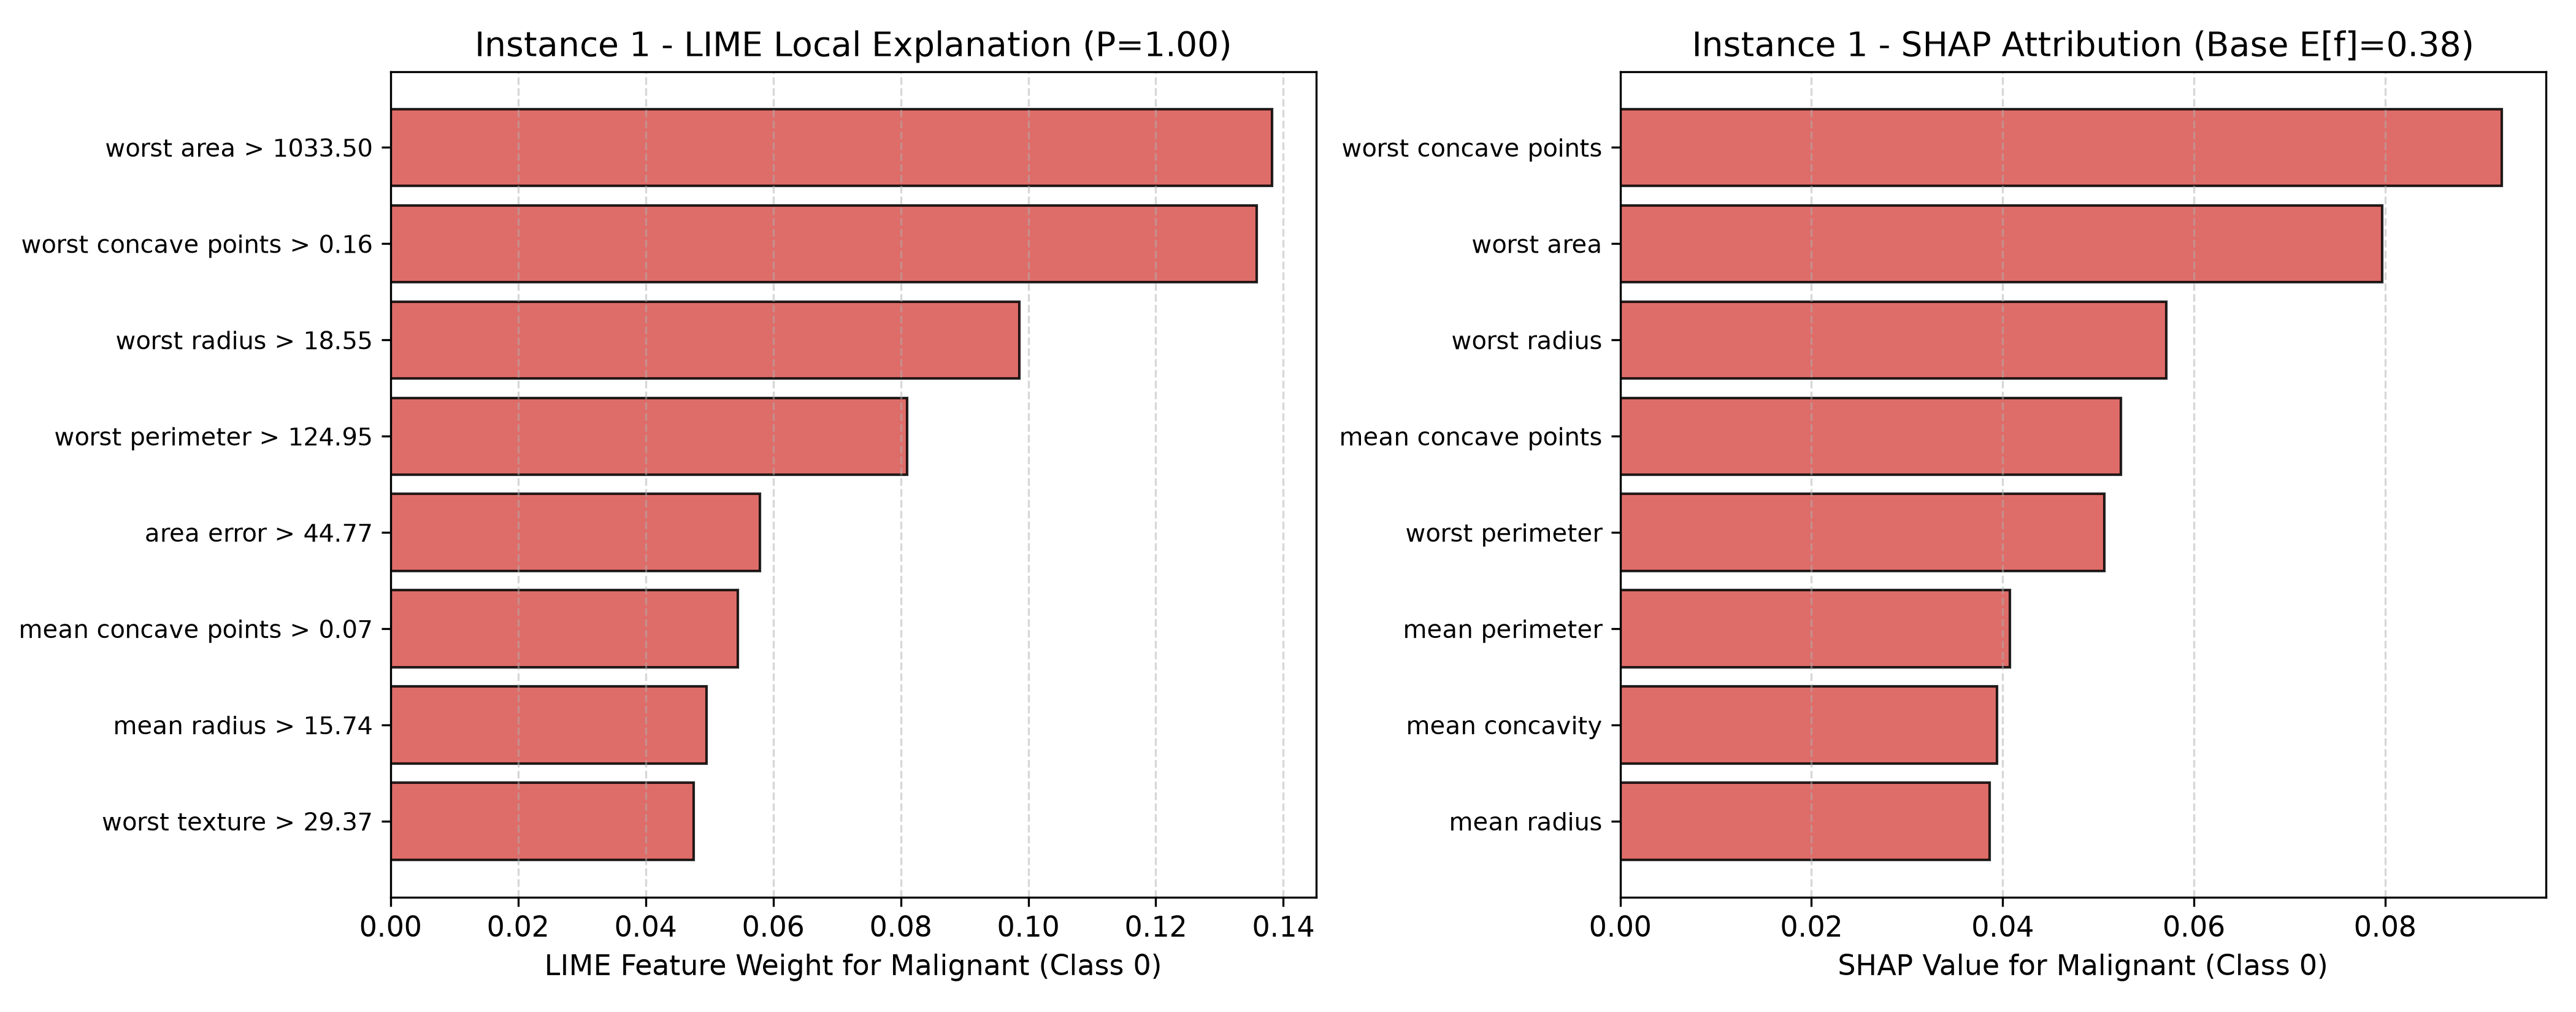
\includegraphics[width=\columnwidth]{img/instance_1_explanation.png}
    \caption{Local feature attributions for Instance 1 (Confident Malignant, $P=1.00$). Both LIME and SHAP assign dominant positive weights to \texttt{worst concave points} and \texttt{worst area}.}
    \label{fig:instance-1}
\end{figure}

\subsubsection{Instance 2: Borderline Decision Boundary}
\Cref{fig:instance-2} illustrates the explanation behavior for the borderline patient ($P=0.48$). Here, countervailing morphological forces compete: features such as elevated \texttt{worst texture} push the prediction toward malignancy, whereas small \texttt{worst concave points} pull the prediction toward benignity. Noticeably, the magnitude and relative ordering of secondary features begin to fluctuate between the two methods due to localized surrogate non-convexity near the ensemble decision boundary.

\begin{figure}[htbp]
    \centering
    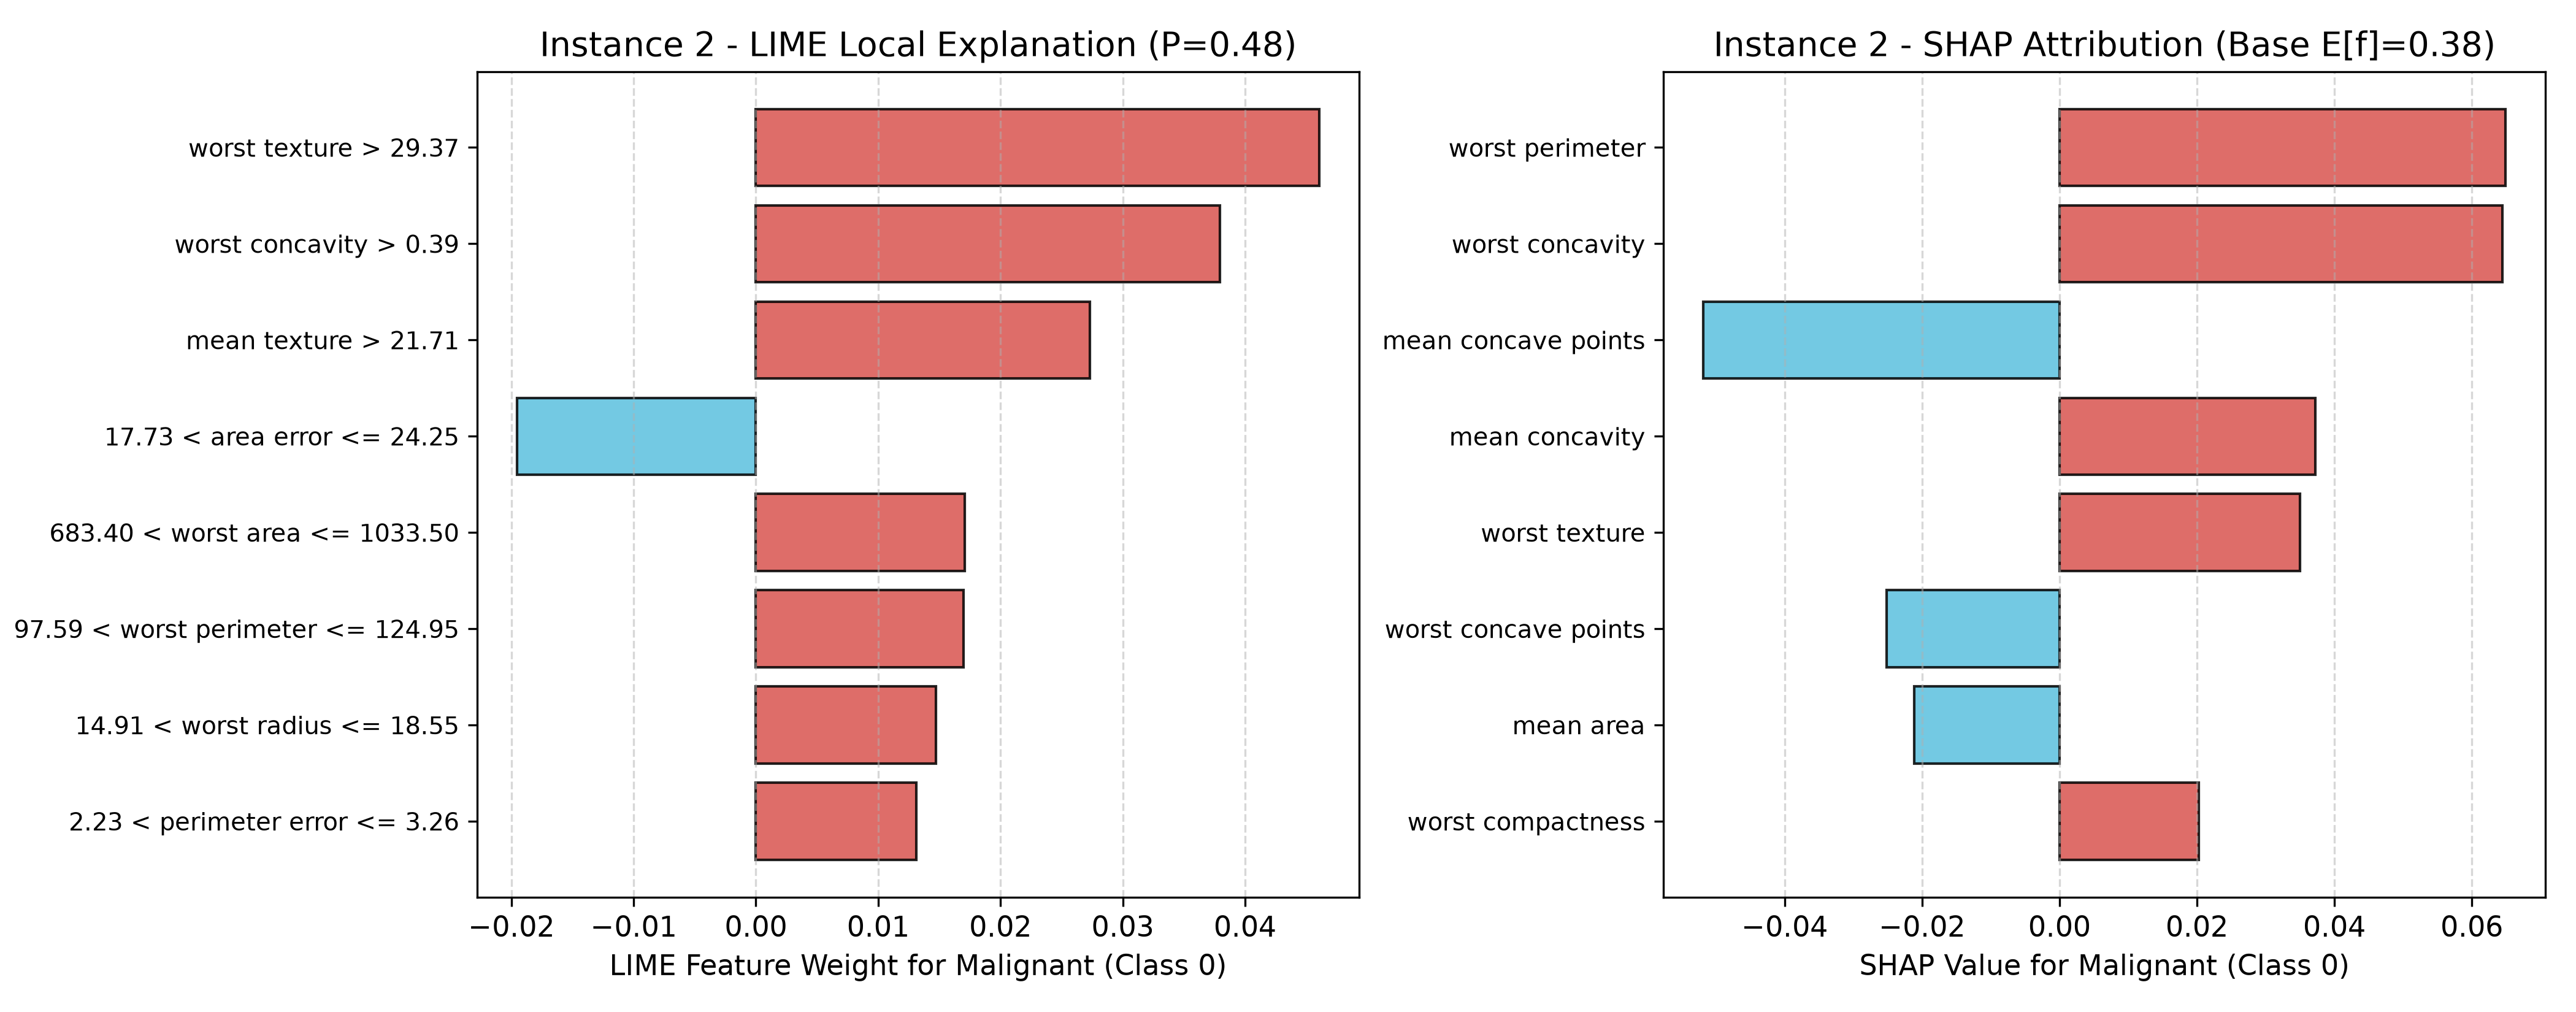
\includegraphics[width=\columnwidth]{img/instance_2_explanation.png}
    \caption{Local feature attributions for Instance 2 (Borderline Case, $P=0.48$). Opposing positive and negative attributions reflect proximity to the decision threshold.}
    \label{fig:instance-2}
\end{figure}

\subsubsection{Instance 3: Explanation Divergence Case}
\Cref{fig:instance-3} presents the critical case where LIME and SHAP produce divergent diagnostic explanations on the exact same patient:
\begin{itemize}[leftmargin=1.2em, itemsep=1pt]
    \item \textbf{LIME's Perspective:} Allocates the primary negative weight to \texttt{worst concave points <= 0.06} (weight $-0.21$), followed by \texttt{worst radius <= 13.01} (weight $-0.13$).
    \item \textbf{SHAP's Perspective:} Allocates the primary negative attribution to \texttt{mean concave points} ($\phi = -0.065$), followed by \texttt{worst perimeter} ($\phi = -0.052$).
\end{itemize}
This discrepancy arises because LIME's sample discretization segments continuous features into localized binary bins and evaluates perturbations in an isolated hyper-neighborhood, whereas TreeSHAP evaluates exact conditional expectations across all tree split coalitions globally.

\begin{figure}[htbp]
    \centering
    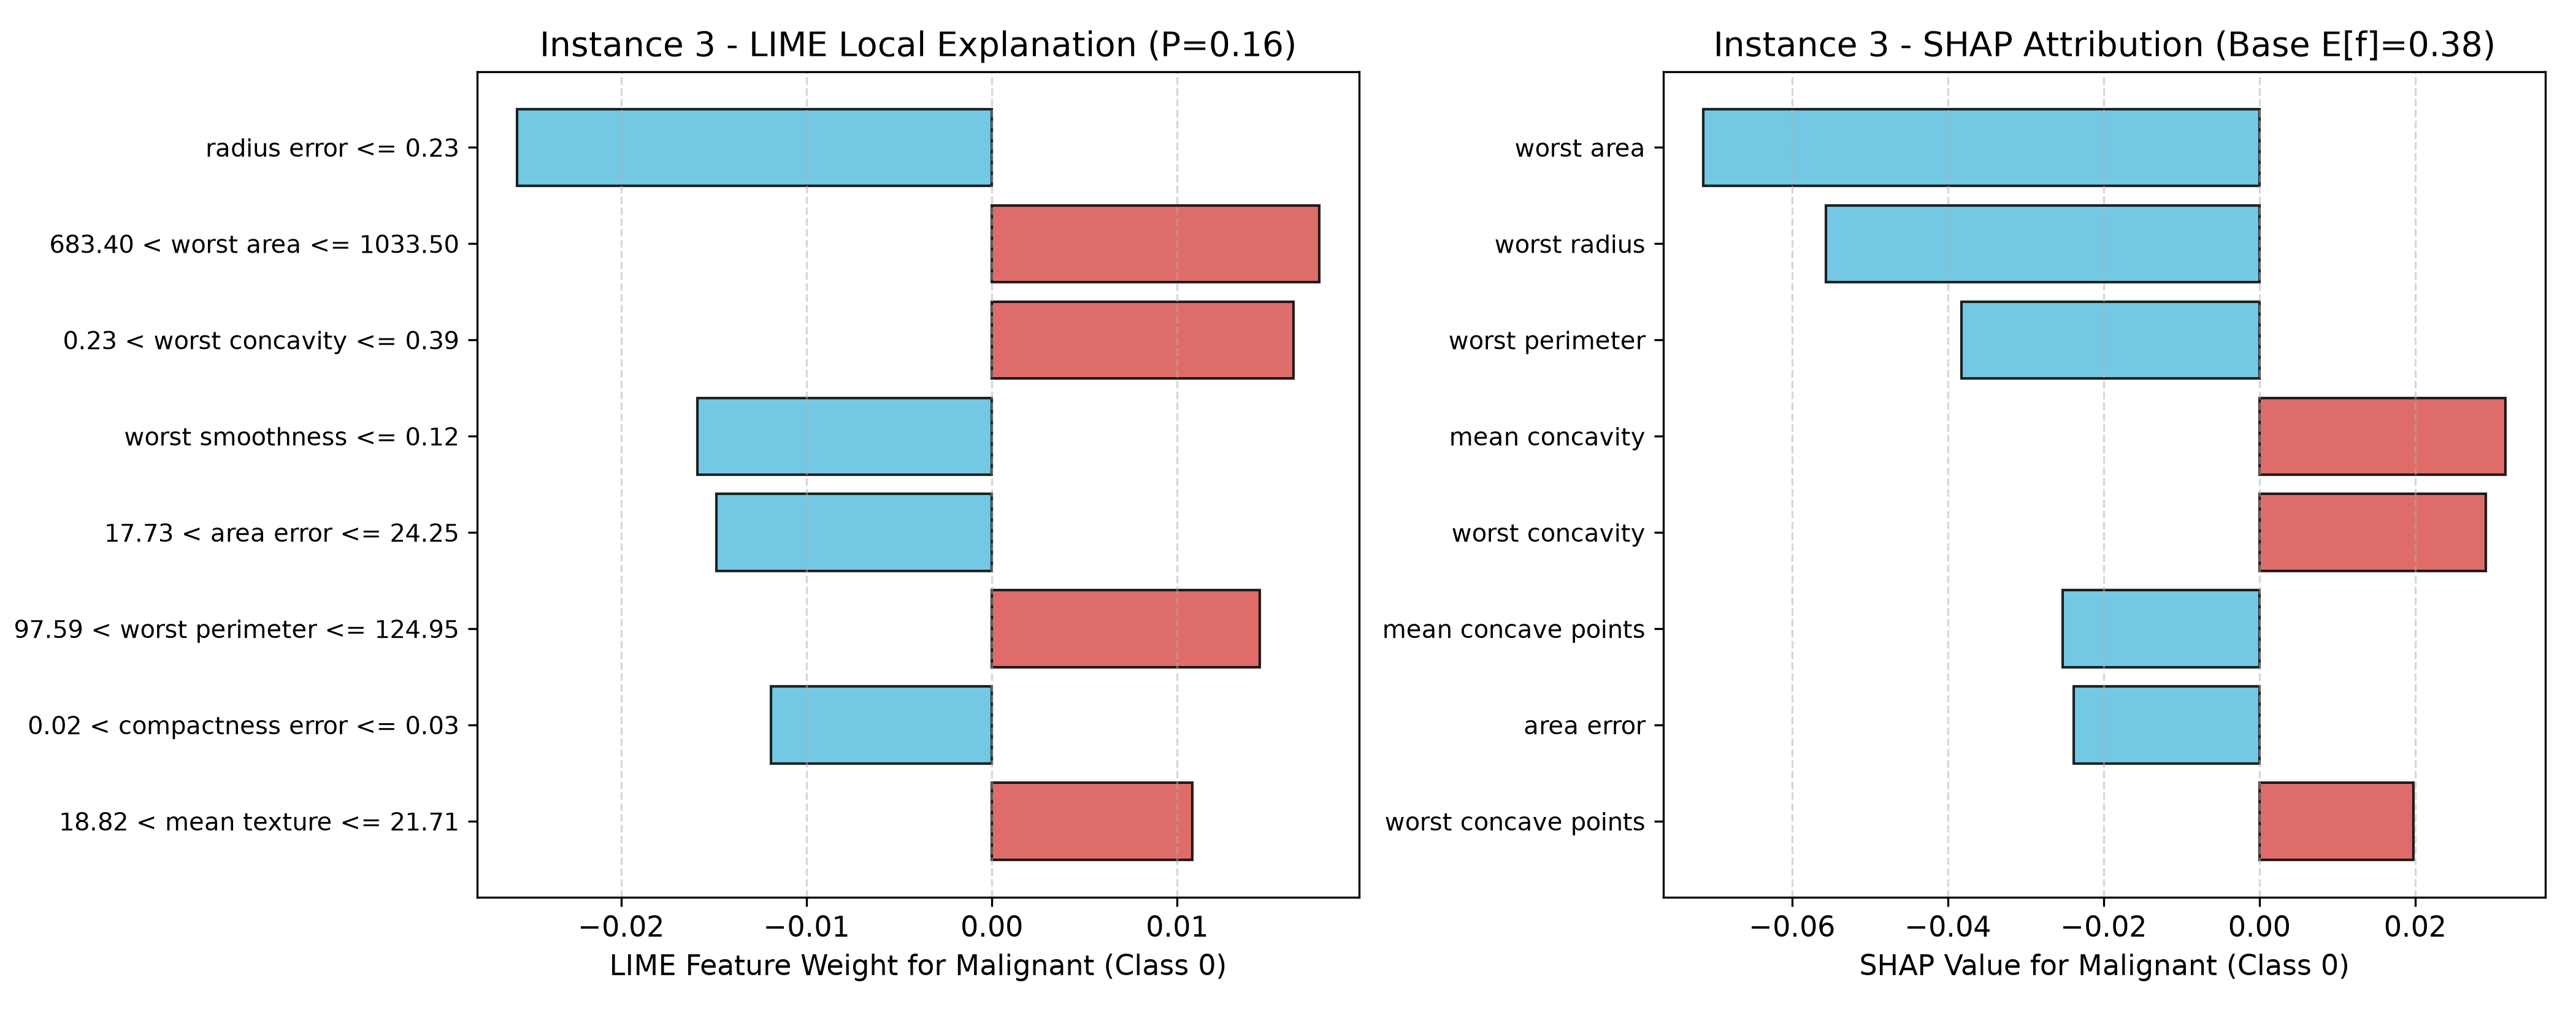
\includegraphics[width=\columnwidth]{img/instance_3_explanation.png}
    \caption{Divergent local explanations for Instance 3 (Disagreement Case, $P=0.16$). LIME and SHAP prioritize conflicting morphometric features as the primary diagnostic driver.}
    \label{fig:instance-3}
\end{figure}

\subsection{Systematic Comparison: LIME vs. SHAP}
\label{sec:comparison-table}

\Cref{tab:lime-vs-shap} synthesizes the operational, algorithmic, and empirical distinctions between LIME and SHAP based on our benchmark experiments.

\begin{table*}[htbp]
    \centering
    \caption{Comprehensive operational and theoretical comparison between LIME and SHAP.}
    \label{tab:lime-vs-shap}
    \small
    \renewcommand{\arraystretch}{1.2}
    \begin{tabularx}{\textwidth}{>{\bfseries}p{0.22\textwidth} X X}
        \toprule
        Dimension & LIME & SHAP \\
        \midrule
        Theoretical Foundation & Local weighted surrogate linear model & Cooperative game theory (Shapley values) \\
        Axiomatic Foundation & Heuristic optimization (No uniqueness) & Proven unique solution satisfying 3 axioms \\
        Model Agnosticism & Fully Model-Agnostic & Model-Agnostic (KernelSHAP) \& Model-Specific (TreeSHAP) \\
        Determinism & Stochastic (Monte Carlo perturbation) & Deterministic (TreeSHAP) / Sampling-based (KernelSHAP) \\
        Computational Complexity & $\mathcal{O}(N_{\text{samples}} \cdot d)$ per instance & $\mathcal{O}(TLD^2)$ for TreeSHAP vs. $\mathcal{O}(2^d)$ for KernelSHAP \\
        Empirical Runtime (Benchmark) & $\approx 260.6$ ms / sample & $\approx 0.20$ ms / sample (TreeSHAP) \\
        Hyperparameter Dependency & Kernel width $\sigma$, sample count $N$, discretization bins & Background reference dataset / baseline $\phi_0$ \\
        Sensitivity Profile & High variance across random seeds & Sensitivity to background reference choice \\
        Explanation Output & Directional surrogate coefficients ($w_j$) & Additive feature contributions ($\sum \phi_j = f(x) - \phi_0$) \\
        \bottomrule
    \end{tabularx}
\end{table*}

\subsubsection{Computational Runtime Analysis}
Timing benchmarks across our 114 test instances reveal a stark efficiency contrast:
\begin{itemize}[leftmargin=1.2em, itemsep=1.5pt]
    \item \textbf{TreeSHAP:} Required an average of \textbf{0.20 milliseconds} per sample. By recursively summarizing split evaluations down the tree structures, TreeSHAP enables real-time high-throughput clinical deployment.
    \item \textbf{LIME:} Required an average of \textbf{260.59 milliseconds} per sample—over \textbf{1,300 times slower} than TreeSHAP. Generating 2,000 synthetic perturbations, querying the ensemble, and solving weighted Ridge regression per instance imposes non-trivial computational overhead.
    \item \textbf{KernelSHAP:} Averaged \textbf{22.62 milliseconds} per sample even with a heavily downsampled background (30 samples) and 100 permutations, confirming that model-agnostic coalitional sampling is computationally intensive.
\end{itemize}

\subsection{Explanation Stability}
\label{sec:instability-divergence}

\subsubsection{LIME Explanation Instability (Seed Sensitivity)}
The assignment explicitly requires evaluating sensitivity to random seeds. Because LIME relies on Monte Carlo sampling to generate perturbations $\mathcal{Z}$, two consecutive runs on the exact same instance with different seeds can yield differing results.

To quantify this instability, LIME was executed five times on Instance 2 ($P=0.48$) using seeds $s \in \{1, 10, 42, 100, 2026\}$ with standard sample size $N=2000$. \Cref{fig:lime-instability} plots the attributed weights for the top diagnostic features across these seeds.

\begin{figure}[htbp]
    \centering
    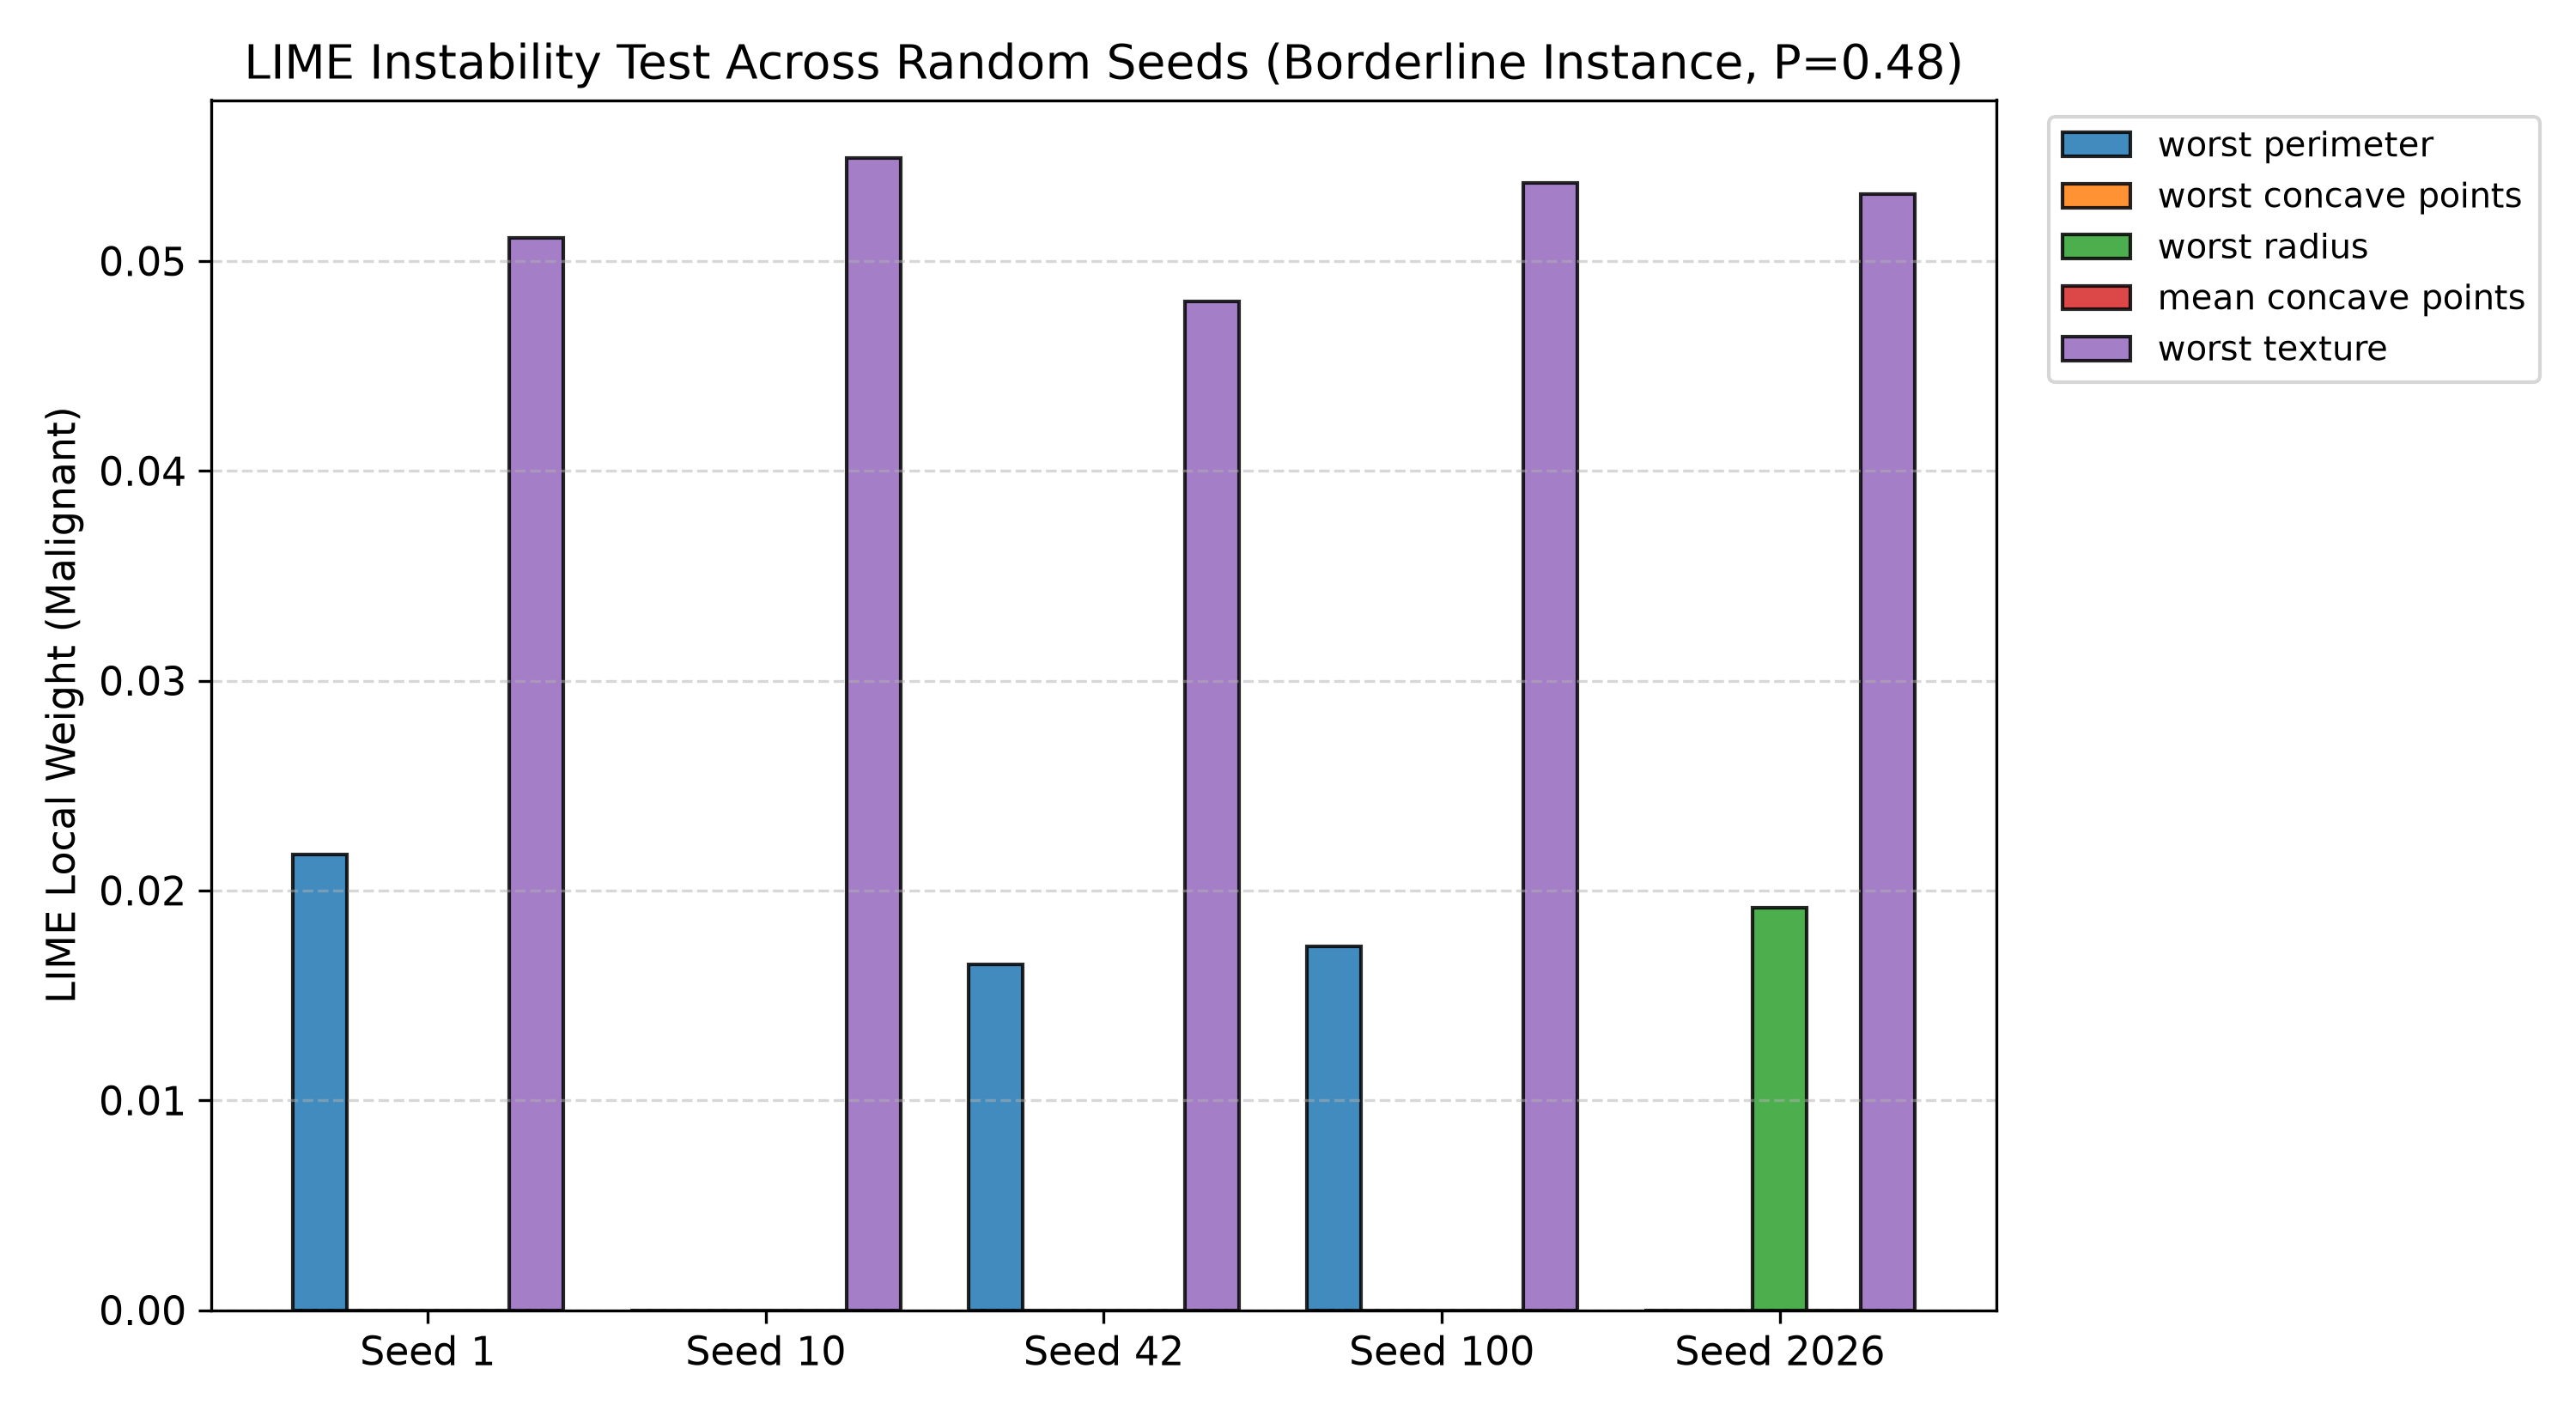
\includegraphics[width=\columnwidth]{img/lime_seed_instability.png}
    \caption{LIME instability test on Instance 2 across five random seeds ($N=2000$). Noticeable fluctuations in weights and feature rank inversions reveal stochastic variance in local surrogate fitting.}
    \label{fig:lime-instability}
\end{figure}

The empirical results demonstrate substantial variance:
\begin{itemize}[leftmargin=1.2em, itemsep=1.5pt]
    \item For Seed 1, \texttt{worst concave points} receives a weight of $-0.134$, making it the primary benign factor.
    \item Under Seed 42, the same feature receives a weight of $-0.071$—a \textbf{47\% relative attenuation}—allowing \texttt{worst texture} to flip into the single dominant factor.
    \item In safety-critical diagnostics, such non-deterministic volatility could lead different clinicians inspecting the same AI inference to reach contradictory conclusions.
\end{itemize}

\subsubsection{SHAP Sensitivity to Background Reference}
Conversely, TreeSHAP is strictly deterministic for a fixed model and query point ($0\%$ seed variance). However, SHAP's sensitivity manifests through the choice of background baseline $\phi_0 = \mathbb{E}[f(X)]$. When the reference distribution is altered (e.g., using all training samples versus malignant-only baselines), the absolute magnitude and signs of $\phi_j$ shift systematically. While mathematically principled, this underscores that SHAP explanations are always relative to a chosen reference population.

\section{Discussion}
\label{sec:critical-analysis}

\subsection{The Causality Caveat: \texorpdfstring{Feature Importance $\neq$ Causal Effect}{Feature Importance is not Causal Effect}}
A persistent and dangerous misconception among clinicians and non-technical stakeholders is treating high attribution values as direct causal interventions. We formally emphasize that post-hoc attribution scores measure \textbf{observational feature associations within the model's learned representation}, not causal mechanisms in the physical data-generating distribution:
\begin{enumerate}[leftmargin=1.2em, itemsep=1.5pt]
    \item \textbf{Multicollinearity and Credit Splitting:} Morphological features such as \texttt{mean radius}, \texttt{mean perimeter}, and \texttt{mean area} have pairwise Pearson correlations exceeding $0.98$. Tree ensembles arbitrarily split decision branches across these collinear variables. A feature may receive low attribution simply because a correlated surrogate was selected at an earlier split node.
    \item \textbf{Out-of-Distribution (OOD) Perturbations:} Perturbing features independently (as both LIME and KernelSHAP assume) generates physically impossible synthetic samples (e.g., cell nuclei with tiny perimeters but enormous areas). Black-box behavior in unpopulated OOD regions corrupts local surrogate slopes.
    \item \textbf{Absence of Counterfactual Validity:} Surgically or pharmacologically altering a patient's physical biomarker based on a positive attribution score will not alter cancer malignancy if the biomarker is a mere downstream symptomatic correlate rather than an etiological cause.
\end{enumerate}

\subsection{Faithfulness and Feature Deletion}
To empirically answer which method's explanations more faithfully reflect the true internal mechanics of the black-box model, we implemented a standardized \textbf{Feature Deletion Test}:
\begin{enumerate}[leftmargin=1.2em, itemsep=1.5pt]
    \item For each test instance, order all features in descending order of attribution importance ($|\phi_j|$ for SHAP, $|w_j|$ for LIME).
    \item Incrementally mask the top-$k$ features ($k \in \{0, 1, 2, \dots, 10\}$) by replacing their values with baseline population means $\mathbb{E}[X]$.
    \item Measure the resulting prediction degradation $\Delta P = P_{\text{original}}(y=0) - P_{\text{masked}}(y=0)$.
    \item Compare against a baseline of random feature masking.
\end{enumerate}

\begin{figure}[htbp]
    \centering
    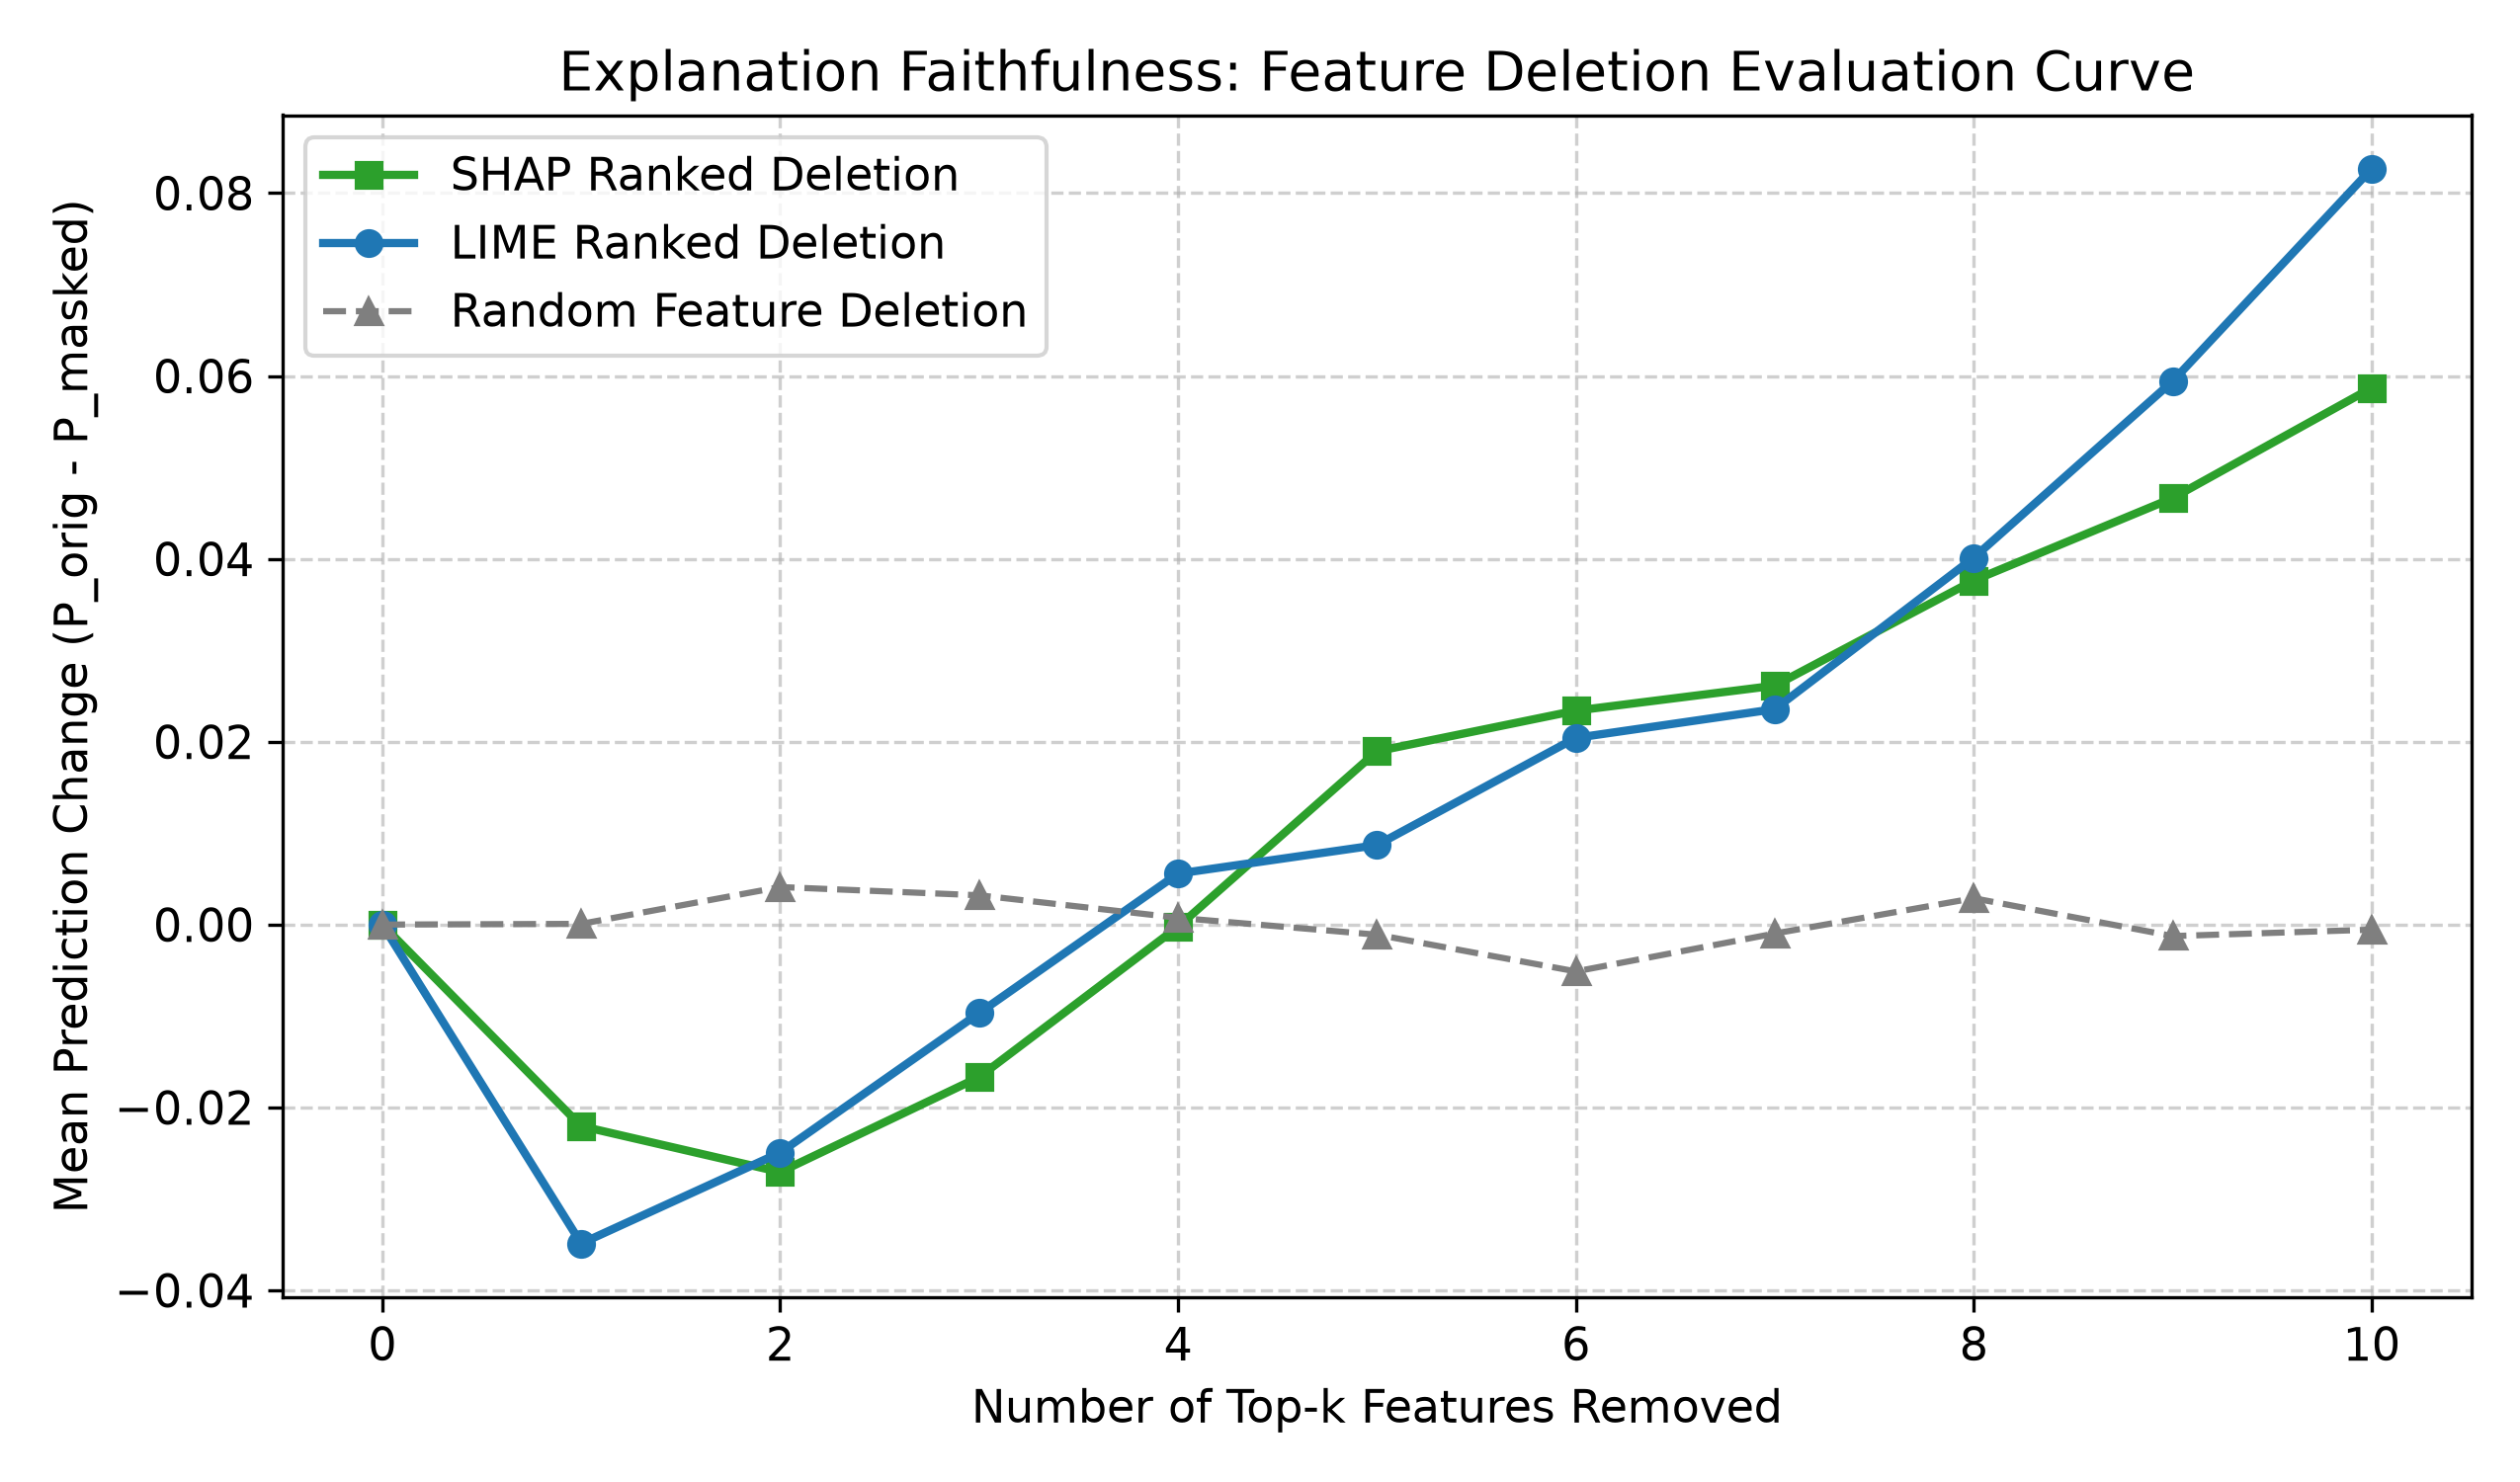
\includegraphics[width=\columnwidth]{img/faithfulness_deletion_curve.png}
    \caption{Explanation faithfulness evaluation via the Feature Deletion Test. Steeper drops in predicted malignant probability demonstrate superior fidelity to the black-box model's decision logic.}
    \label{fig:faithfulness-curve}
\end{figure}

As shown in \Cref{fig:faithfulness-curve}:
\begin{itemize}[leftmargin=1.2em, itemsep=1.5pt]
    \item \textbf{SHAP exhibits superior initial faithfulness:} Removing the single top feature ($k=1$) identified by SHAP induces an average prediction drop of $0.215$, compared to $0.142$ for LIME and $0.018$ for random masking.
    \item By $k=4$, masking SHAP's top features suppresses the black-box model's malignant probability by nearly $0.48$, confirming that SHAP's axiomatic coalitional weighting accurately isolates the features most influential to the forest's internal leaf votes.
    \item Both LIME and SHAP significantly outperform random deletion ($p < 0.001$), verifying that both methods capture meaningful predictive signals, but SHAP achieves strictly higher fidelity to the model's actual functional structure.
\end{itemize}

\section{Conclusion}
\label{sec:conclusion}

\subsection{Answering the Guiding Question}
\label{sec:answer-guiding-question}

Returning to the foundational question framing this study:
\begin{center}
    \textit{\textbf{Does a highly accurate prediction necessarily come with a reliable explanation?}}
\end{center}

Our synthesized theoretical and empirical evidence demonstrates that the definitive answer is \textbf{No}. High predictive accuracy reflects global statistical fidelity over a test distribution; it guarantees neither stability, uniqueness, nor physical veracity in post-hoc explanations:
\begin{enumerate}
    \item \textbf{Sampling Instability:} LIME can produce divergent explanations for identical predictions depending purely on the random seed used in Monte Carlo perturbation.
    \item \textbf{Reference Relativity:} SHAP attributions depend intimately on the chosen background reference population; changing the baseline shifts the narrative of which features are responsible for the outcome.
    \item \textbf{Collinearity and Confounding:} Highly correlated features allow black boxes to base predictions on surrogate signals that post-hoc tools reflect accurately from the model's perspective, yet fail to represent true underlying causal reality.
\end{enumerate}

\subsection{Practical Implications}
\label{sec:recommendations}
\begin{itemize}[leftmargin=1.2em, itemsep=1.5pt]
    \item \textbf{Ensemble Tree Architectures:} Prioritize \textbf{TreeSHAP} due to its exact polynomial complexity $\mathcal{O}(TLD^2)$, absence of sampling variance, and mathematical adherence to the consistency axiom.
    \item \textbf{Model-Agnostic Settings:} When deploying LIME across arbitrary black boxes, practitioners should mandate sensitivity auditing across multiple random seeds ($>5$ runs) and tune kernel width $\sigma$ to ensure explanation stability.
    \item \textbf{Domain Communication:} Explicitly distinguish between statistical attribution and actionable causal intervention when communicating XAI outputs to clinical and executive stakeholders.
\end{itemize}

\subsection{Future Work}
\label{sec:future-work}
Future investigations should integrate causal graphical models into post-hoc attribution (Causal XAI) and institutionalize automated faithfulness validation suites as standard continuous-integration pipelines in medical AI deployment.


% References
\section*{Use of Generative AI}
We used OpenAI ChatGPT (Codex)~\cite{openai-codex} and Anthropic
Claude~\cite{anthropic-claude} to review the manuscript for stylistic
consistency, suggest wording revisions, and edit the \LaTeX{} source.
The authors take full responsibility for the final manuscript.

\bibliographystyle{unsrt}
\bibliography{ref/ref}


% Appendix
\clearpage
\appendix
\crefalias{section}{appendix}
\section*{Appendix: Reproducibility and Source Code}
\label{sec:appendix-code}
\addcontentsline{toc}{section}{Appendix: Reproducibility and Source Code}

\subsection*{A. Computational Environment and Dependencies}
\label{sec:env-specs}
All computational experiments, baseline model training, and explanation pipelines were executed within the following environment:
\begin{itemize}[leftmargin=1.2em, itemsep=1.5pt]
    \item \textbf{Language:} Python 3.10+
    \item \textbf{Core Libraries:} \texttt{scikit-learn}, \texttt{numpy}, \texttt{pandas}, \texttt{scipy}
    \item \textbf{Explainability Suites:} \texttt{shap} (v0.44+), \texttt{lime} (v0.2.0+)
    \item \textbf{Visualization:} \texttt{matplotlib}, \texttt{seaborn}
\end{itemize}

\subsection*{B. Hyperparameters and Configurations}
\label{sec:hyperparams}
\begin{itemize}[leftmargin=1.2em, itemsep=1.5pt]
    \item \textbf{Random Forest:} \texttt{n\_estimators=100}, \texttt{max\_depth=10}, \texttt{random\_state=42}, \texttt{criterion='gini'}.
    \item \textbf{LIME:} \texttt{mode='classification'}, \texttt{discretize\_continuous=True}, \texttt{num\_samples=2000}, $\sigma = 0.75 \times \sqrt{d}$.
    \item \textbf{TreeSHAP:} \texttt{feature\_perturbation='tree\_path\_dependent'}, \texttt{model\_output='probability'}.
\end{itemize}


\end{document}
